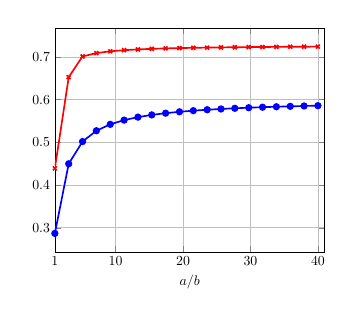
\begin{tikzpicture}[scale=0.5]
\begin{axis}[xlabel=$a/b$,ymajorgrids=true,xmajorgrids=true,xmin=1,xmax=41,xtick={1,10,20,30,40}]
%%%%%%%%%%% NATURAL CONFIGURATION
\addplot[Blue,mark=*,very thick] coordinates {(1.0,0.286705918022) (3.05263157895,0.449716071021) (5.10526315789,0.501782746472) (7.15789473684,0.527153462699) (9.21052631579,0.54213191771) (11.2631578947,0.552009414669) (13.3157894737,0.559009934788) (15.3684210526,0.564229666081) (17.4210526316,0.568271008297) (19.4736842105,0.571492328044) (21.5263157895,0.574120115076) (23.5789473684,0.576304512257) (25.6315789474,0.578148974898) (27.6842105263,0.579727104075) (29.7368421053,0.581092688356) (31.7894736842,0.58228594869) (33.8421052632,0.583337561737) (35.8947368421,0.584271331895) (37.9473684211,0.585106013388) (40.0,0.585856581891) };
%%%%%%%%%%% MODIFIED CONFIGURATION
\addplot[Red,mark=x,very thick] coordinates {(1.0,0.438891399031) (3.05263157895,0.652556925298) (5.10526315789,0.701154248564) (7.15789473684,0.708927502176) (9.21052631579,0.713138668165) (11.2631578947,0.715778473448) (13.3157894737,0.717587786989) (15.3684210526,0.718905133196) (17.4210526316,0.719907103779) (19.4736842105,0.720694821913) (21.5263157895,0.721330359644) (23.5789473684,0.721853926318) (25.6315789474,0.722292713971) (27.6842105263,0.722665770137) (29.7368421053,0.722986834444) (31.7894736842,0.723266066974) (33.8421052632,0.723511142614) (35.8947368421,0.72372796708) (37.9473684211,0.72392115889) (40.0,0.724094381918) };
\end{axis}
\end{tikzpicture}
%%% Local Variables:
%%% mode: latex
%%% TeX-master: "../../mainManuscript"
%%% End:
